%% ------------------------------------------------------------------------- %%
\chapter{Modelagem}
\label{cap:modelagem}

Utilizando-se da base de dados para modelagem descrita na seção "Criação da base para modelagem" (\ref{sec:criacao_da_base_para_modelagem}) - cujas variáveis explicativas foram descritas na seção "Variáveis Explicativas" (\ref{sec:variaveis_explicativas}) e a variável resposta descrita na seção "Variável Resposta" (\ref{sec:variavel_resposta}) - foram aplicados modelos de aprendizado de máquina com o intuito de obter o melhor desempenho para predição da variável resposta utilizando as variáveis explicativas construídas.

Os métodos de aprendizado de máquina utilizados foram a Regressão Linear, o Random Forest e o XGBoost, sendo que a afinação dos parâmetros de tais modelos foi feita utilizando o método Randomized Search. A avaliação de desempenho destes modelos foi feita utilizando-se de duas métricas, a raiz do erro quadrático médio e as bandas de acerto, e a interpretação dos modelos Random Forest e XGBoost foram feitas por meio do método Shapley Value.

\section{Análise Descritiva}
\label{sec:analise_descritiva}

A análise descritiva consiste em explorar dados utilizados para a modelagem com o intuito de encontrar a existência, ou não, de uma relação causal entre as variáveis explicativas e a variável resposta. Neste trabalho já foram apresentados algumas análises descritivas no capítulo \ref{cap:contexto}, como, por exemplo, as estatísticas dos percentuais de polaridade que representam a variável resposta.

Foram utilizadas 52 variáveis explicativas neste trabalho, assim, foi realizado uma verificação em cada uma das variáveis utilizando-se gráficos de dispersão. Nestes gráficos de dispersão, os valores observados para a variável explicativa estão dispostos no eixo das ordenadas e os valores observados para a variável resposta estão dispostos no eixo das abscissas. Como exemplo, abaixo está o gráfico de dispersão da variável 'family_var_01_inappropriate_pct' (que se trata do percentual de domicílios particulares permanentes em situação inadequada por município em 2000 dividido pela mesma informação em 2010), nota-se uma relação linear positiva média entre a variável explicativa e a variável resposta. Os gráficos de dispersão de todas as variáveis explicativas se encontram no anexo \ref{ape:cap2_scatter_plot}.

\graphicspath{ {./figuras/two_by_two_scatter_plot/} }
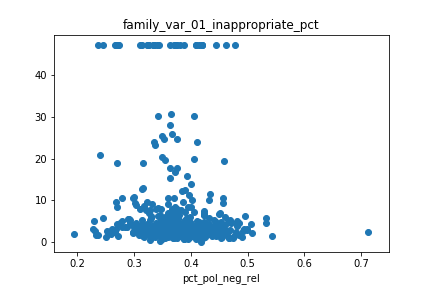
\includegraphics{04_family_var_01_inappropriate_pct}

O código citado no parágrafo anterior foi escrito na linguagem de programação Python utilizando a ferramenta Notebook Jupyter e se encontra no anexo \ref{ape:model_visualization}.

\section{Randomized Search}
\label{sec:randomized_search}

O Randomized Search é um método utilizado para otimização de hiperparâmetros que consiste em uma pesquisa aleatória sobre os hiperparâmetros fornecidos para treinamento de modelos de aprendizado de máquina visando o melhor desempenho de tal modelo. Neste trabalho foi escolhido utilizar-se o Randomized Search frente aos dois métodos mais utilizados na atualidade, o Grid Search (ref.) e a busca manual, uma vez que o Randomized Search realiza buscas mais eficientes que o Grid Search e a busca manual (ref.).

Foi-se utilizada a implementação deste método proveniente do pacote em Python sklearn (ref.). Ao contrário do Grid Search, nem todos os valores dos parâmetros são testados, mas um número fixo de configurações de parâmetros é amostrado das distribuições especificadas. O número de configurações de parâmetros que são tentadas é definido pela quantidade de iterações passadas ao método e o desempenho do modelo de aprendizado de máquina treinado após a escolha dos hiperparâmetros é calculado utilizando-se do método de validação cruzada.

Se todos os parâmetros forem apresentados como uma lista, é realizada a amostragem sem reposição. Se pelo menos um parâmetro for fornecido como distribuição, é utilizada a amostragem com reposição. No âmbito deste trabalho, alguns parâmetros foram fornecidos como lista e outros como distribuição, assim, para o treinamento do modelo de aprendizado de máquina Random Forest foi-se utilizado uma amostragem com reposição e para o treinamento do modelo de aprendizado de máquina XGBoost foi-se utilizado uma amostragem sem reposição.

Além do Randomized Search ser a melhor opção por sua eficiência, existe a motivação da viabilidade da otimização dos hiperparâmetros, uma vez que para o treinamento do modelo de aprendizado de máquina XGBoost foi-se utilizado dez diferentes hiperparâmetros com diferentes quantidades de valores, representando no final uma quantidade de 1.411.200 possibilidades ou cenários distintos para o treinamento.

\section{Shapley Value}
\label{sec:shapley_value}

O Shapley Value é um conceito de solução na teoria dos jogos cooperativos, foi nomeado em homenagem a Lloyd Shapley que o definiu inicialmente (ref.). 

Em um cenário de jogos cooperativos onde, para cada jogo cooperativo, atribui-se uma distribuição única (entre os jogadores) de um excedente total gerado pelo grupo de todos os jogadores, o Shapley Value é caracterizado como uma coleção de propriedades para explicação da proveniência de cada parte desse excedente total.

A configuração é da seguinte forma: um grupo de jogadores coopera e obtém um certo ganho geral com essa cooperação. Como alguns jogadores podem contribuir mais para o grupo do que outros, ou podem ter um poder de barganha diferente, qual a importância de cada jogador para a cooperação geral e que recompensa ele pode razoavelmente esperar? Esta pergunta é uma das motivações para criação do Shapley Value, i.e., explicar essa importância individual e a recompensa esperada.

O paralelo da explicação acima à explicação do algoritmo em aprendizado de máquina (ref.) seria de que os jogadores são as variáveis explicativas, o ganho geral obtido por cada jogador é o impacto na predição do modelo e a importância individual seria a importância da variável explicativa no modelo. A importância das variáveis explicativas em modelos de aprendizado de máquina é uma informação amplamente discutida (ref.), uma vez que existem diferentes formas de serem calculadas, sendo que a ordenação da importância das variáveis podem ser diferentes de um método para outro gerando discussão sobre a escolha do melhor método a ser utilizado (ref.).

O Shapley Value vem sendo considerado uma das formas mais robustas e consistentes de se avaliar a importância das variáveis explicativas (ref.), ele será utilizado neste trabalho tanto para ordenação da importância das variáveis quanto para interpretação do valor das variáveis explicativas. Foi-se utilizada a implementação deste método proveniente do pacote em Python SHAP (ref.).

\section{Regressão Linear}
\label{sec:regressao_linear}

(?).

\section{Random Forest}
\label{sec:random_forest}

(?).

\section{XGBoost}
\label{sec:xgboost}

(?).

%% ------------------------------------------------------------------------- %%